\icode{E-EXM-FI-L2-260625-002}
某同学利用如图所示的实验装置验证机械能守恒定律，弧形轨道末端水平，离地面的高度为\(H\)。将钢球从轨道的不同高度\(h\)处静止释放，钢球的落点距轨道末端的水平距离为\(x\)。
  
(1)若轨道完全光滑，\(x^2\)与\(h\)的理论关系应满足\(x^2 =\)\underline{\hbox to 6em{}}(用\(H\)、\(h\)表示)。

\begin{figure}[htbp]
    \centering
    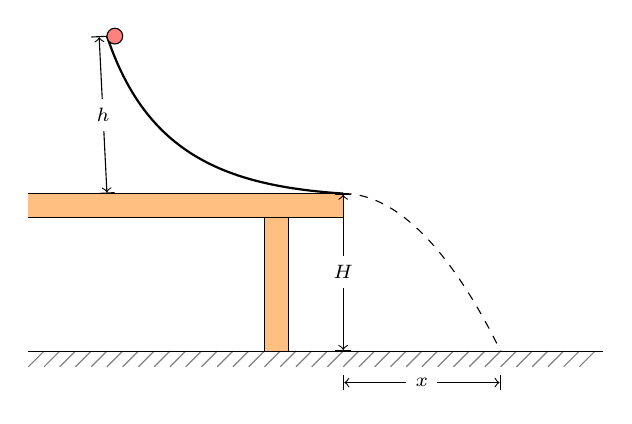
\begin{tikzpicture}
    \filldraw[fill=orange!50] (-4,-.3)--(0,-.3)--(0,0)--(-4,0) (-1,-.3) rectangle(-.7,-2);
    \draw[thick] (-3,2)..controls(-2.5,.5)and(-1.5,.1)..(0,0);
    \draw[fill=red!50] (-2.9,2) circle(.1);
    \draw[|<->|,font=\scriptsize] (-3.1,2)--node[fill=white]{\(h\)}(-3,0);
    \draw[|<->|,font=\scriptsize] (0,0)--node[fill=white]{\(H\)}(0,-2);
    \draw[|<->|,font=\scriptsize] (0,-2.4)--node[fill=white]{\(x\)}(2,-2.4);
    \draw[dashed] (0,0) parabola bend (0,0)(2,-2);
    \foreach \x in {-4,-3.8,...,3}
        \draw[gray] (\x,-2.2)--++(.2,.2);
    \draw (-4,-2)--(3.3,-2);
\end{tikzpicture}
\begin{tikzpicture}[scale=1.2]
    \draw[help lines,color=gray!80,very thin,step=.1] (0,0)grid(3.5,3.5);
    \draw[->,font=\scriptsize,blue] (0,0)--(4.5,0)node[below]{\(h\)/\( \times \)\qty{e-1}{m}};
    \draw[->,font=\scriptsize,blue] (0,0)--(0,4)node[right]{\(x^2\)/\( \times \)\qty{e-1}{m^2}};
    \foreach \x/\y in {.5/1,1/2,1.5/3,2/4,2.5/5,3/6,3.5/7}
        \node at(\x,0)[below,font=\scriptsize,blue]{\(\y\)};
    \foreach \x/\y in {.5/2,1/4,1.5/6,2/8,2.5/10,3/12,3.5/14}
        \node at(0,\x)[left,font=\scriptsize,blue]{\(\y\)};
    \node[font=\scriptsize,blue] at(-.2,-.2) {\(O\)};
    \draw[thin,purple] (0,0)--(3.5,3.5);
    \draw[->,font=\scriptsize,gray] (4,3.5)node[right]{理论}--(3.5,3.5);
    \end{tikzpicture}
\end{figure}

(2)该同学经实验测量得到一组数据，如下表所示：

\begin{table}[ht]
    \centering
    \begin{tblr}{|r|c|c|c|c|c|}
    \hline
    \(h\)/(\(\times\)\qty{e-1}{m})&2.00&3.00&4.00&5.00&6.00\\
    \hline
    \(x^2\)/(\(\times\)\qty{e-1}{m^2})&2.62&3.89&5.20&6.53&7.79\\
    \hline
    \end{tblr}
\end{table}

请在坐标纸上作出\(x^2 - h\)关系图。

(3)对比实验结果与理论计算得到的\(x^2 - h\)关系图线(下图中已画出)，自同一高度静止释放的钢球，水平抛出的速率\underline{\hbox to 3em{}}(填“小于”或“大于”)理论值。

(4)从\(x^2 - h\)关系图线中分析得出钢球水平抛出的速率差十分显著，你认为造成上述偏差的可能原因是\underline{\hbox to .7\textwidth{}}